% Use cases, to be included in requirements.tex

\subsection{Use cases}

Figures \ref{prospective} and \ref{uc_actors} show the use case diagrams.

\subsubsection{A prospective e-Customer registers}
\begin{center}
	\rowcolors{0}{tablerow}{white}
	\begin{tabularx}{\linewidth}{>{\hsize=.3\hsize}r X}
		Actors              & Prospective e-Customer \\
		Goals               & [G0]  \\
		Input conditions    & The Prospective e-Customer is on the home page and wants to start the registration process \\
		Events flow         & 1) The Prospective e-Customer clicks on the “Customer Sign Up” button on the home page \newline
		2) The Prospective e-Customer inserts their new credentials \newline
		3) The Prospective e-Customer clicks on the “Registration” button \newline
		4) The system saves the data \newline
		5) The system shows a message stating that registration ended successfully \\
		Output conditions   & Registration process ended successfully. From now on the new user can use the system as an e-customer \\
		Exceptions          & - Credentials inserted by the Prospective e-Customer are not suitable (e.g. invalid email) \newline
		- Username provided by the Prospective e-Customer is already taken \newline
		\newline
		Exceptions are handled by showing an error message to the Prospective e-Customer to inviting them to restart the registration  process. Event flow restarts from point 2 \\
	\end{tabularx}
\end{center}

\subsubsection{A Prospective Store Manager registers a store}
\begin{center}
	\rowcolors{0}{tablerow}{white}
	\begin{tabularx}{\linewidth}{>{\hsize=.3\hsize}r X}
		Actors              & Prospective Store Manager \\
		Goals               & [G1]  \\
		Input conditions    & The Prospective Store Manager wishes to register their store \\
		Events flow         & 1) The Prospective Store Manager clicks on the “Register a store” button on the home page \newline
		2) The Prospective Store Manager inserts their new credentials \newline
		3) The Prospective Store Manager inserts their store information \newline
		3) The Prospective Store Manager clicks on the “Registration” button \newline
		4) The system saves the data \newline
		5) The system sends an email about the registration \\
		Output conditions   & The registration process ended up successfully. From now on the Store Manager can access their dedicated functions \\
		Exceptions          &  - Credentials or information inserted by the Prospective Store Manager are not suitable (e.g. invalid store address) \newline
		- Username provided by the Prospective Store Manager is already taken \newline
		- The store is already registered \newline
		\newline
		Handled by showing an error message to the Prospective e-Customer to inviting them to restart the registration  process. Event flow restarts from point 2 \\
	\end{tabularx}
\end{center}

\subsubsection{An e-Customer lines up}
\begin{center}
	\rowcolors{0}{tablerow}{white}
	\begin{tabularx}{\linewidth}{>{\hsize=.3\hsize}r X}
		Actors              & e-Customer \\
		Goals               & [G2]  \\
		Input conditions    & e-Customer is already logged in and wants to enqueue \\
		Events flow         & 1) The e-Customer clicks on the "New ticket" button to access the section \newline
		2) The e-Customer inserts current location and mean of trasport \newline
		3) The app searches for available stores and shows them to the e-Customer  \newline
		4) The e-Customer chooses a store and presses "generate" \newline
		5) The system enqueues the e-Customer  for their desired store and generates a QR code for entrance \\
		Output conditions   & The process is concluded correctly and the QR code is saved on the device, under tickets \\
		Exceptions          & - No stores are available for the defined parameters \newline
		Handled by showing an error pop-up asking to check the parameters or try again later  \newline
		- Selection becomes unavailable during the selection \newline
		Handled with an error message \\
	\end{tabularx}
\end{center}

\subsubsection{An e-Customer deletes a ticket}
\begin{center}
	\rowcolors{0}{tablerow}{white}
	\begin{tabularx}{\linewidth}{>{\hsize=.3\hsize}r X}
		Actors              & e-Customer \\
		Goals               & [G2.1]  \\
		Input conditions    & The e-Customer is logged, has an active ticket and wishes to dequeue \\
		Events flow         & 1) The e-Customer accesses the ticket page \newline
		2) The e-Customer presses the "Cancel ticket" button and confirms \\
		Output conditions   & The system updates the queue and shows a confirmation message \\
		Exceptions          &  \\
	\end{tabularx}
\end{center}

\subsubsection{A store manager modifies the store's information}
\begin{center}
	\rowcolors{0}{tablerow}{white}
	\begin{tabularx}{\linewidth}{>{\hsize=.3\hsize}r X}
		Actors              & Store Manager \\
		Goals               & [G3]  \\
		Input conditions    & The Store Manager is logged in and wants to update some information \\
		Events flow         & 1) The Store Manager clicks on the "Modify store" button \newline
		2) The Store Manager modifies the information \newline
		3) The Store Manager clicks on "Update store" \\
		Output conditions   & The system updates the information and presents a message \\
		Exceptions          & - The Store Manager leaves an empty field \newline
		- The Store Manager insert a not well formed field \newline
		\newline
		Both handled with an error message \\
	\end{tabularx}
\end{center}

\subsubsection{An e-Customer goes to the store}
\begin{center}
	\rowcolors{0}{tablerow}{white}
	\begin{tabularx}{\linewidth}{>{\hsize=.3\hsize}r X}
		Actors              & Store Manager, e-Customer \\
		Goals               & [G2] [G3] [G5]  \\
		Input conditions    & The e-Customer is enqueued and received a notification \\
		Events flow         & 1) The e-Customer reaches the store \newline
		2) The e-Customer waits  for his turn outside until his number is reached \newline
		3) The e-Customer shows their QR code to get scanned \newline
		4) The e-Customer is allowed to enter and shops \newline
		5) The system removes the e-Customer from the queue and counts them as inside \newline
		6) The e-Customer shows the QR code and is allowed to exit \\
		Output conditions   & The system removes the e-Customer from inside the store \\
		Exceptions          & - The e-Customer does not enter in their delay window \newline
		The e-Customer won't be allowed to enter and the queue is shifted  \newline
		- The e-Customer tries to scan the wrong QR code \newline
		The e-Customer is notified of the wrong code and is not allowed to enter \\
	\end{tabularx}
\end{center}

\subsubsection{A Physical Customer lines up}
\begin{center}
	\rowcolors{0}{tablerow}{white}
	\begin{tabularx}{\linewidth}{>{\hsize=.3\hsize}r X}
		Actors              & Physical Customer \\
		Goals               & [G4]  \\
		Input conditions    & A customer not registered to the system wants to enter the shop \\
		Events flow         & 1) The Physical Customer requests the ticket to enter the queue \newline
		2) The ticket is printed and the Physical Customer receives it \\
		Output conditions   & The process is concluded correctly and the QR code is printed \\
		Exceptions          & - The Physical Customer cannot enqueue because the shop is closing or there are too many customers in the queue \newline
		\newline
		The system does not allow the customer to enqueue \\
	\end{tabularx}
\end{center}

\subsubsection{A Physical Customer dequeues}
\begin{center}
	\rowcolors{0}{tablerow}{white}
	\begin{tabularx}{\linewidth}{>{\hsize=.3\hsize}r X}
		Actors              & Physical Customer \\
		Goals               & [G4.1]  \\
		Input conditions    & An already enqueued Physical Customer wants to dequeue \\
		Events flow         & 1) The Physical Customer scans the QR-code \newline
		at entrance of the shop by stating their intentions \newline
		2) The Physical Customer exits the queue \\
		Output conditions   & The Physical Customer is successfully dequeued and the system proceeds to clean the ordering of the queue \\
		Exceptions          & - The Physical Customer goes away without scanning the QR-code \newline
		The system manages this exception by keeping the customer in queue until its delay window is expired and then removes it  \\
	\end{tabularx}
\end{center}

\subsubsection{A Physical Customer shops}
\begin{center}
	\rowcolors{0}{tablerow}{white}
	\begin{tabularx}{\linewidth}{>{\hsize=.3\hsize}r X}
		Actors              & Physical Customer, Store manager \\
		Goals               & [G3]  \\
		Input conditions    & The Physical Customer is at the store \\
		Events flow         & 1) The Physical Customer waits for their turn outside \newline
		3) The Physical Customer shows their QR to get scanned \newline
		4) The system removes the Physical Customer from the queue and counts them as inside \newline
		5) Physical Customer is allowed to enter and shops \newline
		6) Physical Customer shows the QR code and is allowed to exit \\
		Output conditions   & The Physical Customer exits and is removed from the store occupation \\
		Exceptions          & - The Physical Customer does not enter in their delay window \newline
		The Physical Customer  won' t be allowed to enter \newline
		- The Physical Customer tries to scan the wrong QR code \newline
		handled by resuming the flow from point 3) \\
	\end{tabularx}
\end{center}

\subsubsection{An e-Customer books a visit}
\begin{center}
	\rowcolors{0}{tablerow}{white}
	\begin{tabularx}{\linewidth}{>{\hsize=.3\hsize}r X}
		Actors              & e-Customer \\
		Goals               & [G5]  \\
		Input conditions    & The e-Customer is logged in and wants to book a visit \\
		Events flow         & 1) The e-Customer enters in the booking section \newline
		2) The e-Customer inserts their mean of transport and their position \newline
		3) The e-Customer inserts the store, the date and the hour he wants to book \newline
		4) The system registers the reservation \\
		Output conditions   & The booking process ended up successfully. From now on the visit is recorded in the database \\
		Exceptions          & - No slots are available for the given parameters \newline
		Handled by asking the eC to insert different parameters  \\
	\end{tabularx}
\end{center}

\subsubsection{An e-Customer deletes a visit}
\begin{center}
	\rowcolors{0}{tablerow}{white}
	\begin{tabularx}{\linewidth}{>{\hsize=.3\hsize}r X}
		Actors              & e-Customer \\
		Goals               & [G5.1]  \\
		Input conditions    & The e-Customer is logged in and wants to delete a visit \\
		Events flow         & 1) The e-Customer enters in the booking section \newline
		2) The e-Customer clicks on the “active visits” button \newline
		3) The system shows the list of active visits \newline
		4) The e-Customer selects the visit they want to delete and clicks on the delete button \newline
		5) The system deletes the visit from the database \\
		Output conditions   & Deletion process ended successfully. From now on the deleted visit is no longer stored in the database \\
		Exceptions          & - There are no active visits \newline
		The system handles this exception by showing an information message and redirects the user to the home page \\
	\end{tabularx}
\end{center}

\subsubsection{An e-Customer changes the ticket after an alternative slot is proposed}
\begin{center}
	\rowcolors{0}{tablerow}{white}
	\begin{tabularx}{\linewidth}{>{\hsize=.3\hsize}r X}
		Actors              & e-Customer \\
		Goals               & [G2]  \\
		Input conditions    & The e-Customer is logged in, already got a ticket and the chosen store's flow is high  \\
		Events flow         & 1) The system computes a series of alternatives based on the e-Customer's choice  \newline
		2) The system presents to the e-Customer the alternatives \newline
		3) The e-Customer chooses an alternative \\
		Output conditions   & The system dequeues the e-Customer from their current queue and adds them to the new one \\
		Exceptions          & - No alternatives are available \newline
		Handled by not showing any alternative \\
	\end{tabularx}
\end{center}

\subsubsection{An e-Customer subscribes to periodic notifications}
\begin{center}
	\rowcolors{0}{tablerow}{white}
	\begin{tabularx}{\linewidth}{>{\hsize=.3\hsize}r X}
		Actors              & e-Customer \\
		Goals               & [G7]  \\
		Input conditions    & The e-Customer is logged in \\
		Events flow         & 1) The e-Customer accesses the set notifications section \newline
		2) The e-Customer sets the notification parameters (i.e. time, store) and confirms \\
		Output conditions   & The e-Customer is now registered to notifications based on their parameters \\
		Exceptions          & - No slots are available for the given parameters \newline
		Handled by asking the e-Customer to insert different parameters  \\
	\end{tabularx}
\end{center}

\subsubsection{An e-Customer unsubscribes from slot notifications}
\begin{center}
	\rowcolors{0}{tablerow}{white}
	\begin{tabularx}{\linewidth}{>{\hsize=.3\hsize}r X}
		Actors              & e-Customer \\
		Goals               & [G7] \\
		Input conditions    & The e-Customer is subscribed to the notification service \\
		Events flow         & 1) The e-Customer enters in the notification section \newline
		2) The e-Customer clicks on the "Active notifications" button \newline
		3) The system shows the active notifications \newline
		4) The e-Customer selects the service that they want to unsubscribe from \newline
		5) The e-Customer clicks on the "Unsubscribe" button \\
		Output conditions   & The process ended up successfully and the e-Customer is no longer subscribed to the notification \\
		Exceptions          & - The e-Customer is not subscribed to any notification service \newline
		Handled by showing an error and redirecting the eC to the notification page \\
	\end{tabularx}
\end{center}

\subsubsection{An e-Customer gets localized}
\begin{center}
	\rowcolors{0}{tablerow}{white}
	\begin{tabularx}{\linewidth}{>{\hsize=.3\hsize}r X}
		Actors              & e-Customer \\
		Goals               & [G2] [G5] [G6] [G7]  \\
		Input conditions    & The e-Customer is logged in and is compiling a form with a "current position" field \\
		Events flow         & 1) The e-Customer reaches the position field \newline
		2) The system obtains the e-Customer's position from the "current position" field, if it is empty the web mapping service is used \\
		Output conditions   & The system knows the e-Customer's position \\
		Exceptions          & - The position inserted can not be found by the web mapping service \newline
		Handled by showing an error message and asking to re-insert the position \\
	\end{tabularx}
\end{center}
\begin{figure}[p]
	\centering	
	{	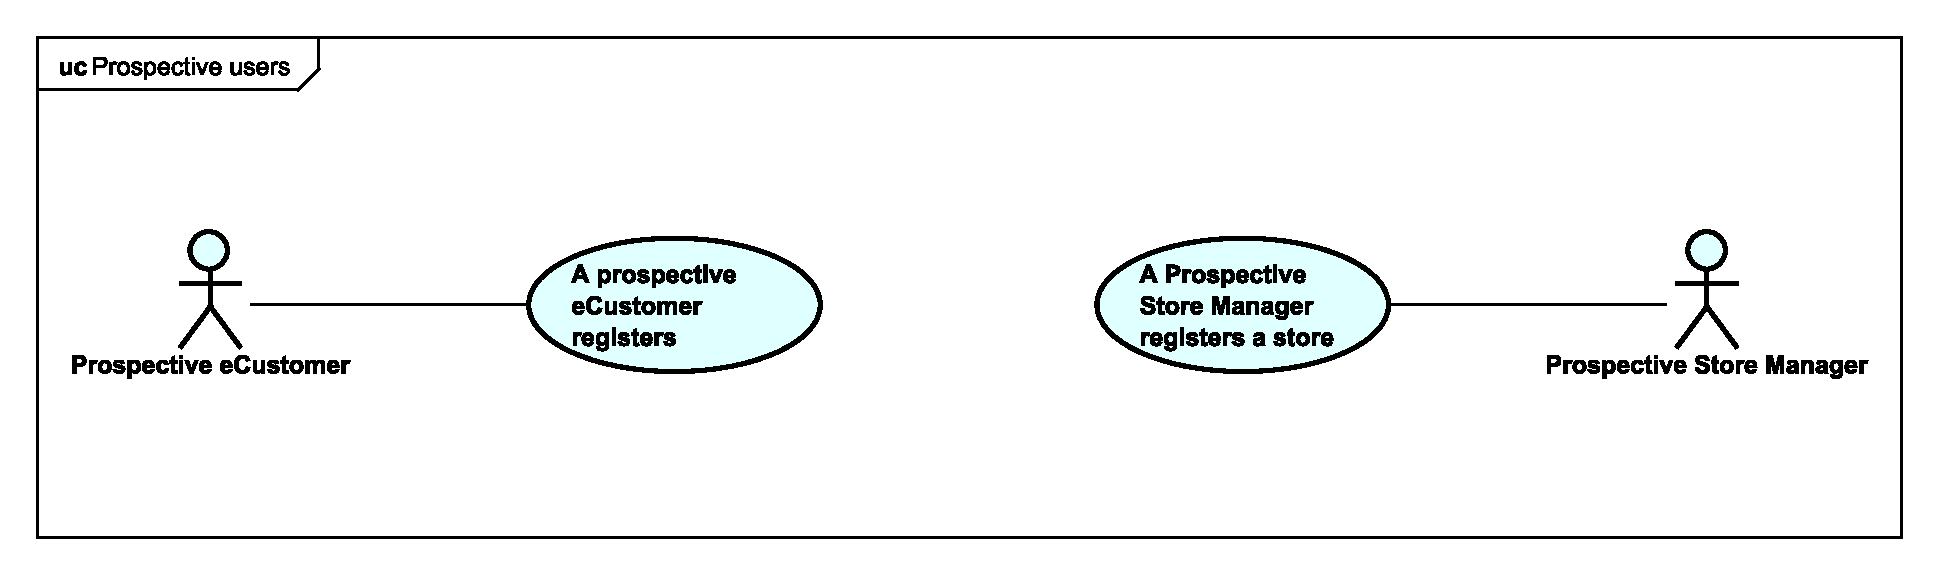
\includegraphics[width=\linewidth] {/use_cases/Prospective_users}
		\caption{Prospective users use cases}
		\label{prospective} }
	{	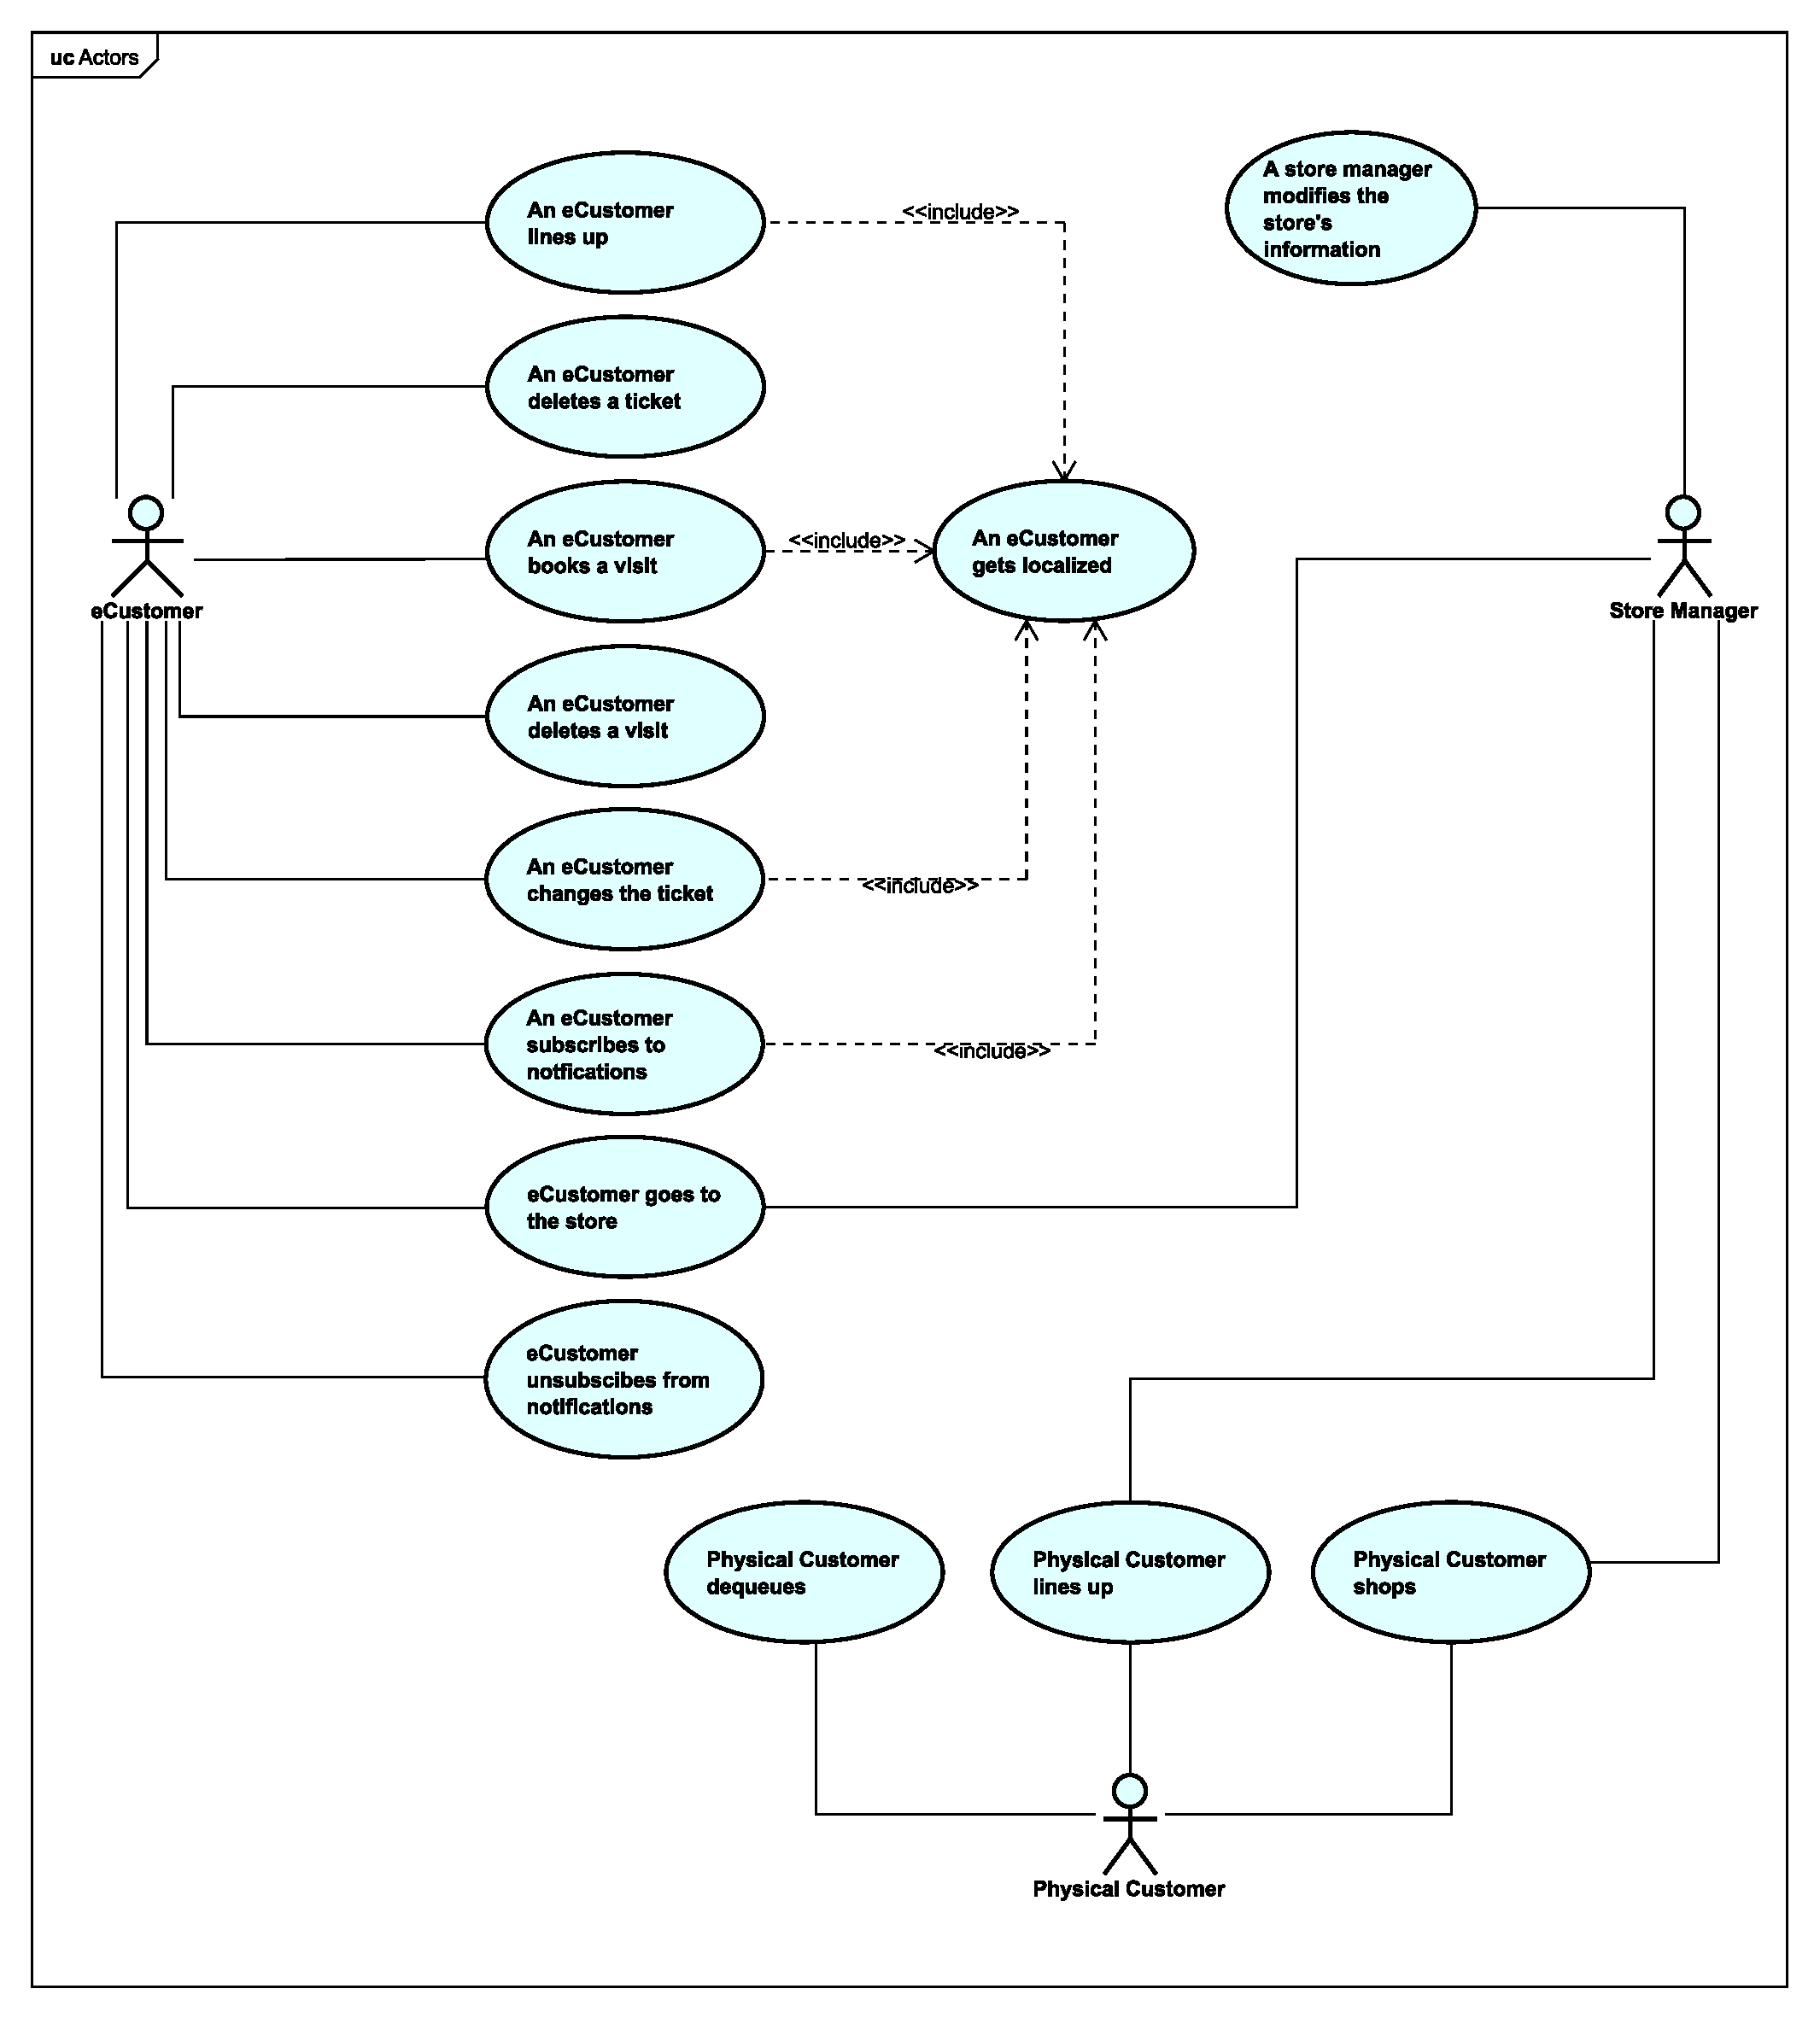
\includegraphics[width=\linewidth] {/use_cases/Actors}
		\caption{Actors use cases}
		\label{uc_actors} }
\end{figure}
\clearpage